\documentclass[11pt, a4paper]{article}

\usepackage{amsmath}
\usepackage{amssymb}
\usepackage{array}
\usepackage{longtable}
\usepackage{multirow}
\usepackage{listings}
\usepackage{xcolor}
\usepackage{siunitx}
\usepackage{seqsplit}
\usepackage{kotex}
\usepackage{booktabs}
\usepackage{caption}
\usepackage{tabularx}
\usepackage{makecell}
\usepackage{float}
\usepackage{graphicx}
\usepackage{titlesec}

\titlespacing*{\section}{0pt}{1.5ex plus 0.5ex minus 0.2ex}{0.8ex plus 0.2ex}
\titlespacing*{\subsection}{0pt}{1.2ex plus 0.4ex minus 0.2ex}{0.5ex plus 0.1ex}
\titlespacing*{\subsubsection}{0pt}{1.0ex plus 0.3ex minus 0.1ex}{0.3ex plus 0.1ex}

\usepackage{fontspec}
\setmainfont{Noto Serif CJK KR}

\usepackage{geometry}
\geometry{margin=0.5in}

\usepackage{hyperref}
\hypersetup{
    colorlinks=true,
    linkcolor=blue,
    urlcolor=blue,
    citecolor=blue
}

\title{MIMIC 기반 기존 연구 리뷰 및 재현 보고서}
\author{2024404060 강민혁}
\date{}

\begin{document}

\maketitle

\section{서론}
\subsection{선택한 논문의 기본 정보}

본 보고서에서 다루는 논문의 제목은 \textbf{``A New Evaluation Model for Traumatic Severe Pneumothorax Based on Interpretable Machine Learning''}이다~\cite{li2024}. 저자는 Jing Li, Yinzhen Lv, Jiayi Weng, Wei Chen, He Huang, Yuzhuo Zhao로 구성되어 있으며, 본 논문은 2024년 \textit{International Journal of Computers Communications \& Control}에 게재되었다. 위 논문은 MIMIC-IV 데이터셋을 기반으로 머신러닝 기법들을 활용하여 외상성 중증 기흉을 신속하고 해석 가능하게 평가하는 모델을 제안한 연구이다.

\subsection{선택 이유 및 연구 주제의 중요성}
외상성 기흉은 신속한 진단이 생존율에 직결되는 응급 질환으로, 영상 검사가 어려운 환경에서도 활용 가능한 예측 모델의 임상적 필요성이 높아 본 연구를 선정하였다. 특히, 해석 가능한 머신러닝을 통해 임상적 타당성을 확보한 점과 MIMIC-IV 데이터를 활용한 재현 가능성이 본 과제의 학습 목표와 부합하여 적절하다고 판단하였다.

\section{기존 논문 리뷰}
\subsection{연구 목적}
해당 연구는 중환자실 임상 데이터베이스인 MIMIC-IV를 활용하여 외상성 중증 기흉을 신속하게 진단하고 평가할 수 있는, 해석 가능한 머신러닝 기반의 새로운 평가 모델을 제안하는 것을 주된 목적으로 한다. 레퍼런스 논문의 저자들은 기존의 영상 의학적 진단 방식이 응급 상황, 대량 사상자가 발생하는 재난 상황, 혹은 의료 자원이 부족한 환경에서 신속한 대응이 어렵다는 한계점에 주목하였다. 이에 대한 대안으로 영상 검사 결과가 도출되기 전, 환자의 활력 징후와 혈액 가스 분석 등에서 추출한 12가지 주요 임상 변수를 활용하여 기흉의 중증도를 조기에 판별할 수 있는 데이터 기반 모델을 구축하였다.

해당 연구는 XGBoost, ANN, SVM, KNN 등 네 가지 머신러닝 알고리즘의 예측 성능을 비교 분석하여 외상성 기흉 평가에 최적화된 알고리즘을 도출하고자 하였으며, SHAP을 통해 헤모글로빈, 산소화 지수, pH 등 핵심 인자가 모델의 예측 결과에 미치는 영향을 정량적으로 규명하고 임상적 타당성을 확보하는 데 중점을 두었다. 나아가 eICU 데이터셋을 활용한 외부 검증을 수행함으로써 제안된 모델의 강건성과 일반화 가능성을 입증하고자 하였다.

\subsection{데이터 및 코호트 정의}
해당 연구는 MIMIC-IV를 기반으로 하였다. 연구 대상자는 성인 환자 중 인구통계학적 정보와 병원 진료 기록이 온전한 환자로 한정하였으며, 분석의 신뢰도를 높이기 위해 폐질환 및 심장질환 등 기흉 발생이나 호흡기 지표에 영향을 줄 수 있는 기저 질환을 보유한 환자를 제외하였다. 또한, 데이터의 결측률이 50\% 이상이거나 이상치가 포함된 샘플 역시 분석에서 배제하였다.

코호트는 외상성 중증 기흉 환자로 구성된 실험군과 비외상성 비기흉 환자로 구성된 대조군으로 분류하였다. 실험군은 외상으로 입원한 환자 중 CXR에서 대형 기흉(흉벽에서 폐 외연까지 2cm 이상 등)이 확인되었거나 흉강 천자, 흉관 삽입술 등 기흉 치료를 받은 환자 174명으로 정의하였다. 대조군은 외상 및 기흉 소견이 없고 폐 관련 수술 이력이 없으며 생존 퇴원한 환자 3,697명이 포함되었다. 이때, 데이터 불균형 문제를 해소하기 위해 대조군에 대해 1:5 비율의 다운샘플링을 적용하였다.

예측 모델 구축을 위한 변수로는 활력 징후와 혈액 가스 분석 지표 33개를 1차적으로 추출하였다. 이 중 임상적 중요도와 결측률(50\% 미만 기준)을 고려하여 최종적으로 pH, Hemoglobin, PaO$_2$, Lactate, Oxygenation Index, SpO$_2$, Base Excess, Heart Rate, PaCO$_2$, Systolic BP, Diastolic BP, Respiratory Rate의 12개 핵심 변수를 선별하였다. 각 변수의 상세 정의는 Appendix ``예측 모델에 사용된 변수 정의'' 절에 수록하였다. 선별된 데이터의 결측치는 다중 대체법을 적용하여 보정하였다.

\subsection{기존 연구 결과}
기존 연구 결과, Figure~\ref{fig:original_results}의 좌측 표와 같이 4가지 기계학습 알고리즘 중 XGBoost가 가장 우수한 진단 성능을 보였다. MIMIC-IV 데이터셋을 기반으로 한 내부 검증에서 XGBoost는 AUROC 0.979 (95\% CI: 0.966-0.989), 정확도 0.947, 재현율 0.730을 기록하며 ANN, SVM, KNN 등 타 모델을 전반적으로 상회하는 성능을 입증하였다. 또한, EICU 데이터셋을 활용한 외부 검증에서도 타 모델들과 다르게 XGBoost는 AUROC 0.806을 기록하며 데이터셋 변화에 대해서도 상대적으로 강건한 일반화 성능을 유지하였다.

SHAP 결과는 Figure~\ref{fig:original_results}의 우측 그래프와 같다. 분석 결과, 외상성 중증 기흉 판별에 가장 큰 영향을 미치는 상위 3가지 주요 인자는 pH, Hemoglobin, PaO$_2$인 것으로 확인되었다. 이 세 가지 인자의 수치가 낮을수록 모델이 기흉 위험도를 높게 평가하는 경향을 보였다. 이는 외상성 기흉 환자에게서 나타나는 병태생리학적 특징인 다량의 출혈, 호흡 부전으로 인한 저산소 및 산증과 임상적으로 일치하는 결과이다. 반면 Lactate 수치는 높을수록 기흉의 가능성을 높게 예측하는 주요 인자로 확인되었다.

\begin{figure}[htbp]
  \centering
  \includegraphics[width=1.0\textwidth]{figures/original_results.png}
  \caption{Original Research Performance Evaluation and SHAP Analysis Results. (Left) Model Performance Comparison Table for MIMIC-IV Internal Validation and EICU External Validation. (Right) SHAP Summary Plot for XGBoost Model, showing pH, Hgb, PO2 as the most influential factors in prediction.}
  \label{fig:original_results}
\end{figure}

\section{재현 방법}

\subsection{코호트 구성}
원 논문에서는 MIMIC-IV 데이터베이스로부터 실험군 174명, 대조군 3,697명을 추출하였다고 보고하였다. 본 재현 연구에서는 원 논문에서 기술한 선정 기준을 최대한 준수하여 코호트를 재구성하였으나, Table~\ref{tab:cohort_comparison}과 같이 최종 코호트 규모에서 차이가 발생하였다.

\begin{table}[htbp]
  \centering
  \small
  \caption{Original Study vs. Reproduction Study Cohort Composition}
  \label{tab:cohort_comparison}
  \renewcommand{\arraystretch}{1.2}
  \begin{tabular}{l c c c}
    \toprule
    \textbf{Group} & \textbf{Original Study} & \textbf{Reproduction (Initial)} & \textbf{Reproduction (Final)} \\
    \midrule
    Experimental & 174 & 195 & 119 \\
    Control & 3,697 & 10,174 & 544 \\
    \midrule
    Total & 3,871 & 10,369 & 663 \\
    \bottomrule
  \end{tabular}
  \footnotesize
  \vspace{0.5em}
  
  \textit{Note: Initial extraction yielded 195 experimental and 10,174 control patients. After applying ICU admission requirement, feature extraction constraints, and missing data thresholds, final cohort was reduced significantly.}
\end{table}

실험군 선정 과정에서 본 재현 연구는 ICD-10 진단코드 기반으로 외상성 기흉 및 긴장성 기흉 진단을 받은 환자를 1차적으로 추출하였다. 이후 MIMIC-CXR 데이터베이스의 CheXpert 라벨과 NegBio 라벨을 활용하여 기흉 소견이 양성(Positive)으로 분류된 환자를 선별하였으며, CXR 리포트 원문에 대한 텍스트 마이닝을 추가 수행하여 ``large pneumothorax'', ``tension pneumothorax'', ``chest tube'' 등의 중증도 관련 키워드 또는 2cm 이상의 크기 기술이 포함된 경우를 중증 기흉으로 분류하였다. 또한, 흉관 삽입술 등 기흉 관련 시술 기록이 존재하는 환자도 실험군에 포함하였다. 그러나 원 논문에서는 영상 검사에서 ``흉벽에서 폐 외연까지 2cm 이상'' 또는 ``정점에서 cupola까지 3cm 이상''이라는 구체적인 측정 기준을 제시하였다. 본 재현 과제에서는 컴퓨팅 리소스의 제약 등의 한계로 실제 영상에 대한 직접적인 측정이 불가능하여, CheXpert/NegBio 라벨 및 CXR 리포트의 텍스트 기반 추론에 의존하였다. 이러한 방법론적 차이로 인해 초기 추출된 실험군 195명 중 중증도 확인이 불가능하거나 ICU 입실 기록이 없는 환자가 제외되어 최종 119명으로 감소하였다.

대조군의 경우, 원 논문에서 제시한 기준인 비외상 환자, 기흉 소견 없음, 폐 관련 수술 없음, 생존 퇴원을 적용하여 초기 10,174명을 추출하였다. 이때 CheXpert 및 NegBio 라벨에서 기흉 관련 소견이 음성인 환자만을 대조군 후보로 선정하였다. 그러나 12개 핵심 변수의 결측률 기준을 적용하는 과정에서 상당수가 제외되어 고유 환자 기준 최종 544명만이 분석에 포함되었다.

임상 변수 추출을 위한 시간 윈도우는 실험군과 대조군에 대해 차등적으로 설정하였다. 실험군의 경우 기흉 관련 시술 시간을 기준 시점으로 하되, 시술 시간이 기록되지 않은 경우 ICU 입실 시간, 그것도 없는 경우 입원 시간을 순차적으로 적용하여 기준 시점으로부터 1시간 이전까지의 데이터를 수집하였다. 대조군의 경우에는 퇴원 시간을 기준으로 24시간 이전까지의 데이터를 수집하였다. 이러한 설정을 통해 실험군에서는 급성 기흉 발생 직전의 임상 상태를, 대조군에서는 안정적인 퇴원 전 상태를 반영하고자 하였다.

\subsection{데이터 전처리 파이프라인}
본 재현 연구에서는 원 논문에서 최종 선별된 12개 변수의 유효성을 검증하고, 데이터 추출 과정의 완결성을 높이기 위해 초기 후보 변수군을 확장하였다. 원 논문의 12개 변수에 FiO$_2$와 MAP를 추가하여 pH, Hemoglobin, PaO$_2$, Lactate, SpO$_2$, Base Excess, Heart Rate, PaCO$_2$, DBP, SBP, Respiratory Rate, FiO$_2$, MAP, Oxygenation Index, 총 14개의 변수를 수집하였다. 주요 예측 인자인 Oxygenation Index의 정확한 산출을 위해서 초기 변수 목록을 확장하였다. MIMIC-IV 데이터베이스 특성상 Oxygenation Index가 직접 기록되지 않은 레코드가 존재할 수 있으며, 이 경우 Appendix의 ``수식 정의'' 절에 기술된 산소화 지수 공식을 통해 결측치를 보완하거나 값을 검증해야 하기에 구성 요소인 FiO$_2$와 MAP의 수집이 필수적이었다.

수집된 변수들의 결측률을 산출한 후, 결측률 50\% 초과 변수를 기준으로, 결측 패턴에 높은 가중치를 부여하였으며, 가중치를 기준으로 우선적으로 제거 대상 샘플을 선정하도록 하였다. 구체적으로, 대조군에 대해서는 50\%, 실험군에 대해서는 85\%의 결측률 임계값을 차등 적용하여, 상대적으로 희소한 실험군 샘플을 최대한 보존하면서 분석 품질을 확보하고자 하였다.

기존 연구에서는 결측치 보정을 위해 다중대체법을 사용했다고 서술하였지만, 어떠한 알고리즘을 사용했는지에 대해서는 서술하지 않았다. 이에 본 과제에서는 유사한 일련의 연구에서 다중대체법으로 많이 사용되어왔던 MICE를 활용하였다. 5회의 반복 대체를 수행한 후 평균값을 최종 대체값으로 사용하였다. 최종 모델링 단계에서는 원 논문과의 비교 가능성을 위해 계산 목적으로 사용된 FiO$_2$와 MAP를 제외하고, 핵심 12개 변수만을 입력값으로 확정하였다.

\subsection{베이스라인 모델 및 하이퍼파라미터}
본 과제의 베이스라인 모델은 기존 연구에서 가장 좋은 성능을 냈던 XGBoost로 채택하였다. 이때, 기존 연구와 동일하게 이진 로지스틱 손실 함수를 목적 함수로 설정하였으며, 1:5 다운샘플링을 적용하였다. 이때, 대조군은 무작위 샘플링으로 선정하였다.

그리드 서치를 통해 하이퍼파라미터를 탐색하였다. 단, 기존 연구에서 하이퍼파라미터 후보값을 기재하지 않아 후보값은 임의로 선정하였으며, 선정한 후보값은 Table~\ref{tab:hyperparameters_baseline}과 같다. 총 972개의 조합에 대해 5-Fold 교차 검증을 수행하였다. 각 폴드에서 AUROC를 기준으로 평가하여 가장 높은 평균 AUROC를 달성한 하이퍼파라미터 조합을 최종 모델 구성에 사용하였다.

평가 지표는 기존 연구와 동일하게 Accuracy, F1 Score, Precision, Recall, AUROC, AUPRC, Sensitivity를 사용하였다.

\begin{table}[htbp]
  \centering
  \small
  \caption{Baseline Model XGBoost Hyperparameter Search Range and Optimal Values}
  \vspace{-0.5em}
  \label{tab:hyperparameters_baseline}
  \renewcommand{\arraystretch}{0.85}
  \begin{tabular}{l c l l}
    \toprule
    \textbf{Hyperparameter} & \textbf{Symbol} & \textbf{Search Range} & \textbf{Optimal Value} \\
    \midrule
    Number of Estimators & $M$ & $\{100, 200, 300\}$ & 100 \\
    Max Depth & $d_{\max}$ & $\{3, 5, 7\}$ & 5 \\
    Learning Rate & $\eta$ & $\{0.01, 0.05, 0.1\}$ & 0.05 \\
    Subsample Ratio & $r_{\text{sub}}$ & $\{0.8, 1.0\}$ & 0.8 \\
    Column Subsample Ratio & $r_{\text{col}}$ & $\{0.8, 1.0\}$ & 1.0 \\
    Min Child Weight & $w_{\min}$ & $\{1, 3, 5\}$ & 1 \\
    Min Split Loss & $\gamma$ & $\{0, 0.1, 0.2\}$ & 0.2 \\
    \bottomrule
  \end{tabular}
\end{table}

\subsection{제안 모델 파이프라인}

베이스라인 모델의 낮은 재현율 문제를 극복하고, 임상적 안전성을 확보하기 위해 민감도 최적화에 중점을 둔 개선된 파이프라인을 설계하였다. 데이터셋의 불균형과 제한된 양성 샘플 수를 고려하여, 모델의 일반화 성능 검증에는 5-Fold 교차 검증을 사용하였다. 최종 성능 지표는 기존 논문과 같이 AUROC, AUPRC, Accuracy, F1-score, Sensitivity, Specificity, PPV를 중점적으로 평가하였다.

\subsubsection{재현율 최적화 하이퍼파라미터 튜닝}
양성 클래스에 대한 탐지 능력을 강화하기 위해 기존의 단순 비율 기반 가중치보다 더욱 공격적인 가중치 전략을 적용하였다. 클래스 불균형 해소를 위해 음성/양성 클래스 비율에 기반한 기본값에 2배의 가중치를 추가로 적용하여 설정하였다. 모델의 하이퍼파라미터 최적화는 베이지안 최적화 프레임워크인 Optuna~\cite{akiba2019optuna}를 사용하되, 단일 지표 최적화 시 발생할 수 있는 낮은 재현율 문제를 방지하기 위해, 본 과제에서는 AUROC에 재현율 가중치를 결합한 목적 함수를 구성하였다. 구체적으로는 모델의 판별력을 기본으로 하되, 거짓 음성을 줄이는 것이 중요한 과제 특성을 반영하여 Appendix의 ``수식 정의'' 절에 기술된 복합 목적 함수와 같이 재현율에 $\alpha$의 가중치를 부여하였다. 이때, 가중치 $\alpha$는 0.5로 설정하였으며, 탐색 공간 또한 재현율 향상에 유리하도록, 더 세밀한 결정 경계를 형성할 수 있는 낮은 $w_{\min}$과 $\gamma$ 범위를 포함하도록 조정하였다.

\begin{table}[htbp]
  \centering
  \small
  \caption{Proposed Model XGBoost Hyperparameters via Bayesian Optimization}
  \vspace{-0.5em}
  \label{tab:hyperparameters_proposed}
  \renewcommand{\arraystretch}{0.85}
  \begin{tabular}{l c l}
    \toprule
    \textbf{Hyperparameter} & \textbf{Symbol} & \textbf{Optimal Value} \\
    \midrule
    Number of Estimators & $M$ & 327 \\
    Max Depth & $d_{\max}$ & 10 \\
    Learning Rate & $\eta$ & 0.0117 \\
    Subsample Ratio & $r_{\text{sub}}$ & 0.959 \\
    Column Subsample Ratio & $r_{\text{col}}$ & 0.627 \\
    Min Child Weight & $w_{\min}$ & 2 \\
    Min Split Loss & $\gamma$ & 0.0096 \\
    L1 Regularization & $\alpha_{\text{reg}}$ & 0.0029 \\
    L2 Regularization & $\lambda_{\text{reg}}$ & $3.22 \times 10^{-8}$ \\
    \bottomrule
  \end{tabular}
\end{table}

\subsubsection{제약 조건 기반 임계값 최적화}
모델의 최종 예측 단계에서는 임상적 안전성을 보장하기 위한 제약 조건 기반 임계값 최적화 알고리즘을 적용하였다. 최적의 임계값 $t^*$는 Appendix의 ``수식 정의'' 절에 기술된 최소 민감도 제약과 최소 정확도 제약을 만족하는 범위 내에서 결정되었다. 위 두 조건을 동시에 만족하는 후보 임계값들 중에서 F1-score를 최대화하는 값을 최종 임계값으로 선정하였다. 만약 두 조건을 동시에 만족하는 임계값이 존재하지 않을 경우, 정확도 제약을 일부 완화하고 민감도를 우선시하는 Fallback Policy를 적용하여 기흉 진행 환자의 조기 발견 가능성을 최우선으로 확보하였다.

\subsection{실행 환경}
본 과제의 모든 실험은 X86환경의 Linux 환경에서 수행되었으며, 하드웨어는 AMD Ryzen 9 5900X, 64GB RAM, 그리고 NVIDIA GeForce RTX 3080 GPU로 구성되었다. 데이터 전처리, 모델 학습 및 결과 시각화를 위해 사용된 주요 소프트웨어 라이브러리의 버전은 함께 제출한 Appendix.pdf의 '소프트웨어 환경 및 버전' 절에 기재되어 있으며, 전체 소스 코드는 GitHub\footnote{\url{https://github.com/ga111o/mimic-pneumothorax-progression-analysis}}에서 확인할 수 있다.

\section{실험 결과}
\subsection{성능 지표 비교}
Table~\ref{tab:performance}는 원 논문, 베이스라인 재현 모델, 그리고 제안 모델의 성능을 비교한 결과이다. 베이스라인 모델은 기존 논문의 방법론을 따라 그리드 서치와 1:5 다운샘플링을 적용한 반면, 제안 모델은 앞서 서술했던 Recall 향상에 중점을 둔 파이프라인을 적용하였다.

\begin{table}[H]
\centering
\caption{Diagnostic Performance of Machine Learning Models in Original Study and Reproduction}
\vspace{-0.5em}
\label{tab:performance}
\renewcommand{\arraystretch}{0.85}
\resizebox{\textwidth}{!}{
  \begin{tabular}{llccccccc}
  \toprule
  Model & Dataset & Accuracy & \makecell{F1\\Score} & Precision & Recall & \makecell{AUROC\\(95\% CI)} & AUPRC & Sensitivity \\
  \midrule
  \multicolumn{9}{l}{\textbf{Original Study}} \\
  XGBoost & MIMIC-IV & 0.947 & 0.822 & 0.941 & 0.730 & \makecell{0.979\\(0.966, 0.989)} & 0.926 & 0.991 \\
  \midrule
  \multicolumn{9}{l}{\textbf{Reproduction - Baseline}} \\
  XGBoost & MIMIC-IV & \makecell{0.885\\$\pm$ 0.016} & \makecell{0.557\\$\pm$ 0.076} & \makecell{0.779\\$\pm$ 0.083} & \makecell{0.442\\$\pm$ 0.082} & \makecell{0.910\\$\pm$ 0.038} & \makecell{0.764\\$\pm$ 0.066} & \makecell{0.442\\$\pm$ 0.082} \\
  \midrule
  \multicolumn{9}{l}{\textbf{Proposed Model}} \\
  XGBoost & MIMIC-IV & \makecell{0.883\\$\pm$ 0.034} & \makecell{0.668\\$\pm$ 0.083} & \makecell{0.650\\$\pm$ 0.116} & \makecell{0.700\\$\pm$ 0.100} & \makecell{0.904\\$\pm$ 0.040} & \makecell{0.704\\$\pm$ 0.095} & \makecell{0.700\\$\pm$ 0.100} \\
  \bottomrule
  \end{tabular}%
}
\end{table}

\subsection{제약 조건 기반 임계값 최적화 결과}
제안 모델에서 제약 조건 기반 임계값 최적화를 수행한 결과, 최적 임계값은 0.650으로 결정되었다. 이는 최소 민감도 제약($\text{Recall} \ge 0.45$)과 최소 정확도 제약($\text{Accuracy} \ge 0.85$)을 동시에 만족하면서 F1-score를 최대화하는 지점이다.

Table~\ref{tab:optimized_threshold}는 최적 임계값(0.650)에서의 5-Fold 교차 검증 결과를 보여준다. 베이스라인 대비 Recall이 0.442에서 0.700으로 약 58\% 향상되었으며, F1-score 또한 0.557에서 0.668로 약 20\% 개선되었다.

\begin{table}[H]
\centering
\caption{Cross-Validation Results at Optimized Threshold (0.650)}
\vspace{-0.5em}
\label{tab:optimized_threshold}
\renewcommand{\arraystretch}{0.85}
\begin{tabular}{lc}
  \toprule
  \textbf{Metric} & \textbf{Value (Mean $\pm$ Std)} \\
  \midrule
  AUROC & 0.904 $\pm$ 0.040 \\
  AUPRC & 0.704 $\pm$ 0.095 \\
  Accuracy & 0.883 $\pm$ 0.034 \\
  F1 Score & 0.668 $\pm$ 0.083 \\
  Precision & 0.650 $\pm$ 0.116 \\
  Recall & 0.700 $\pm$ 0.100 \\
  Specificity & 0.920 $\pm$ 0.038 \\
  PPV & 0.650 $\pm$ 0.116 \\
  NPV & 0.939 $\pm$ 0.019 \\
  \bottomrule
\end{tabular}
\end{table}

높은 NPV(0.939)는 모델이 음성으로 예측한 경우 실제로 기흉이 아닐 확률이 매우 높음을 의미하며, 이는 임상적으로 안전한 선별 검사에 적합함을 시사한다. 또한, Recall 0.700은 기흉 진행 환자 10명 중 7명을 정확히 탐지할 수 있음을 의미하여, 베이스라인(0.442) 대비 임상적 안전성이 크게 향상되었다.

\subsection{베이스라인 대비 성능 개선}
Table~\ref{tab:improvement}는 베이스라인 모델과 제안 모델의 주요 지표 비교 결과이다. 제안 모델은 Recall과 F1-score에서 유의미한 개선을 달성하였으며, AUROC와 Accuracy는 소폭 감소하였으나 임상적으로 수용 가능한 수준을 유지하였다.

\begin{table}[H]
\centering
\caption{Performance Comparison: Baseline vs. Recall-Optimized Model}
\label{tab:improvement}
\renewcommand{\arraystretch}{0.85}
\begin{tabular}{lccc}
  \toprule
  \textbf{Metric} & \textbf{Baseline} & \textbf{Proposed} & \textbf{Change} \\
  \midrule
  AUROC & 0.910 & 0.904 & -0.006 \\
  AUPRC & 0.764 & 0.704 & -0.060 \\
  Accuracy & 0.885 & 0.883 & -0.002 \\
  F1 Score & 0.557 & 0.668 & \textbf{+0.111} \\
  Precision & 0.779 & 0.650 & -0.129 \\
  Recall & 0.442 & 0.700 & \textbf{+0.258} \\
  \bottomrule
\end{tabular}
\end{table}

Recall이 0.442에서 0.700으로 약 58\% 향상되었다. 이를 통해 기흉 진행 환자를 놓치는 경우가 크게 줄었다는 것을 확인할 수 있다. 즉, 임상적으로 위험한 환자를 조기에 발견할 가능성이 높아졌음을 시사한다. 단, 이로 인해 Precision이 감소하여 거짓 양성이 증가하였지만, 기존에 알려져 있던 대로 의료 환경에서는 거짓 음성이 거짓 양성보다 더 중요한 지표이기에 이는 문제가 되지 않는다고 판단하였다.

\subsection{SHAP 변수 중요도 분석}
SHAP을 통해 제시한 모델의 예측에 기여하는 주요 변수들을 확인하였다. Table~\ref{tab:shap}은 상위 10개 변수의 평균 SHAP 값을 제시한다.

\begin{table}[H]
\centering
\caption{Top 10 Feature Importance by SHAP Values (Recall-Optimized Model)}
\vspace{-0.5em}
\label{tab:shap}
\renewcommand{\arraystretch}{0.85}
\begin{tabular}{clc}
  \toprule
  \textbf{Rank} & \textbf{Feature} & \textbf{Mean |SHAP|} \\
  \midrule
  1 & Hemoglobin & 0.628 \\
  2 & MAP & 0.447 \\
  3 & PaO$_2$ & 0.404 \\
  4 & Lactate & 0.395 \\
  5 & SpO$_2$ & 0.379 \\
  6 & Oxygenation Index & 0.351 \\
  7 & FiO$_2$ & 0.350 \\
  8 & Base Excess & 0.332 \\
  9 & Systolic BP & 0.301 \\
  10 & Heart Rate & 0.242 \\
  \bottomrule
\end{tabular}
\end{table}

원 논문과 마찬가지로 Hemoglobin이 가장 중요한 예측 인자로 확인되었으며, 이는 외상성 기흉 환자에서 나타나는 출혈과 관련된 병태생리학적 특징과 일치한다. 민감도 최적화 모델에서는 산소화 관련 지표인 PaO$_2$가 3위로 상승하였고, Lactate와 SpO$_2$의 중요도가 높아졌다. 민감도 최적화 과정에서 모델이 호흡 기능 및 조직 관류 상태를 더욱 중요하게 고려하도록 학습되었음을 시사한다. 다만, 기존 논문에서 가장 중요했던 pH는 본 분석에서도 상위 10개에 포함되지 않았다.

\subsection{결과 시각화}
ROC curve, PR curve, SHAP summary plot 등의 시각화 결과는 본 보고서와 함께 제출한 Appendix.pdf에 수록되어 있다.

\subsection{주요 예측 인자에 따른 영상 비교}
SHAP 분석 결과 Hemoglobin이 외상성 중증 기흉 예측에 가장 중요한 인자로 확인되었다. 이러한 결과의 임상적 타당성을 검증하기 위해 Figure~\ref{fig:chest_comparison}와 같이 실험군 내에서 헤모글로빈 수치에 따른 상위 0.5\%, 중위값(50\%), 하위 0.5\%에 해당하는 환자의 흉부 X선 영상을 비교 분석하였다.

\begin{figure}[htbp]
  \centering
  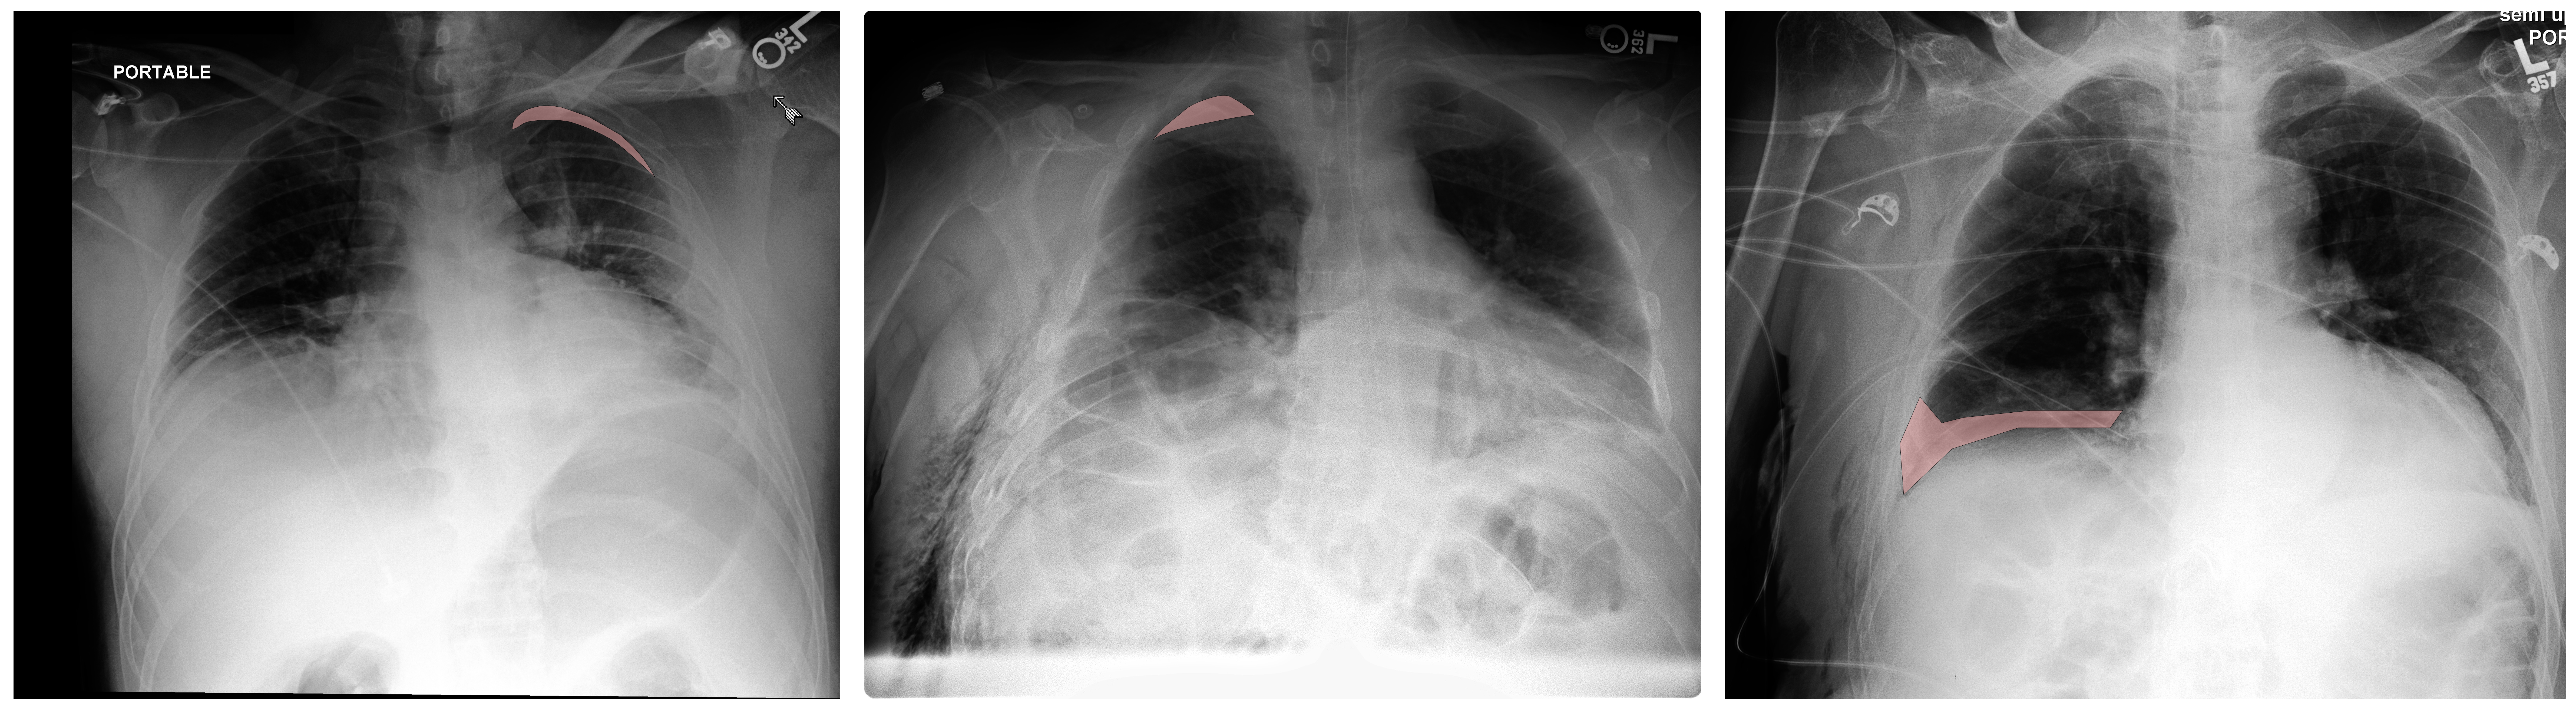
\includegraphics[width=1.0\textwidth]{figures/chest_pa_comparison.png}
  \vspace{-0.5em}
  \caption{Chest X-ray Comparison by Hemoglobin Levels in Traumatic Pneumothorax Patients. Left: High hemoglobin (13.3 g/dL, top 0.5\%), Center: Median hemoglobin (10.77 g/dL), Right: Low hemoglobin (7.15 g/dL, bottom 0.5\%).}
  \label{fig:chest_comparison}
\end{figure}

\paragraph{상위 백분위수 환자 (헤모글로빈 13.3 g/dL)}
LUL상단 용적이 감소한 것을 확인할 수 있다. 동시에 cardiomegaly가 확인되며, heart failure 치료를 위한 diuretics사용으로 hemoconcentration가 일어나 헤모글로빈 수치가 상대적으로 높아진 것으로 파악된다.

\paragraph{중위 백분위수 환자 (헤모글로빈 10.77 g/dL)}
RUL상단 용적이 감수한 것을 확인할 수 있다. 우측 상복부에는 피하 기종이 파악되며, adynamic ileus가 예상된다. 헤모글로빈 수치 자체는는 임상적으로 경도의 빈혈에 해당하나, 본 데이터셋 내에서는 중위값에 해당한다. 즉, 외상성 기흉 환자군 전반에서 출혈에 따른 헤모글로빈 저하가 흔함을 확인할 수 있으며, 원인은 다양하게 나타남을 예상할 수 있다.

\paragraph{하위 백분위수 환자 (헤모글로빈 7.15 g/dL)}
multiple rib fractures 이후 산소포화도 저하와 산소 요구량 증가를 보인 환자이다. rib fractures로 인해 헤모글로빈 수치 감소가 되었음을 예상할 수 있으며, 이와같이 직접적인 외상으로 기흉, 정확히는, Hemo-pneumothorax가 발생함을 확인할 수 있었다.

\paragraph{임상적 해석} 하위 백분위수 환자의 경우, multiple rib fractures과 같은 큰손상이 동반되었으며, 이에 따른 hemothorax로 인해 헤모글로빈 수치의 급격한 저하를 유발한 것으로 판단된다. 이는 헤모글로빈 수치가 외상성 기흉의 중증도와 직결되는 출혈량 및 손상 범위를 대변한다는 점을 시사한다. 반면, 상위 백분위수 환자군에서는 cardiomegaly가 확인되며, diuretics 사용으로 인해 hemoconcentration가 일어나 수치가 높게 측정된 것으로 예상되며, 기저 질환이 있는 환자군에서의 특이적 양상으로 해석할 수 있다. 단, 헤모글로빈 수치가 기흉의 중증도 자체를 대변하기 어렵다는 것을 확인할 수 있었다.

즉, SHAP에서 헤모글로빈이 최상위 예측 인자로 도출된 것은 외상으로 인한 직접적인 출혈과 환자의 기저 상태가 중증 기흉의 예후 및 양상을 결정짓는 핵심 요인이기 때문으로 판단된다. 본 분석에서 사용된 샘플은 각 레벨에서의 하나의 Chest PA만을 가져온 것으로 일반화를 하기에는 한계가 존재하나, 헤모글로빈 수치가 외상성 기흉 환자의 중증도 분류 및 예후 예측에 있어 생리학적으로 타당한 지표임을 뒷받침할 수 있을 가능성을 시사한다.

단, 영상 분석은 레벨에 대해 각각 샘플 하나씩만을 분석한 것으로, 일반화를 하기에는 한계가 존재한다.

\section{논의}
본 과제에서는 원 논문의 주요 결과를 완전히 재현하는 데 한계가 있었다. Table~\ref{tab:performance}에서 확인할 수 있듯이, 베이스라인 재현 모델의 AUROC는 0.910으로 원 논문(0.979)에 비해 약 0.07 낮았으며, Recall은 0.442로 원 논문(0.730)에 비해 약 0.29 낮은 성능을 보였다. 본 절에서는 이러한 성능 차이의 원인과 과제의 한계점을 분석한다.

\subsection{재현 실패 요인 분석}

\paragraph{코호트 구성의 불일치}
가장 근본적인 재현 실패 요인은 코호트 구성의 차이로 판단하였다. 원 논문에서는 실험군 174명, 대조군 3,697명을 추출하였다고 보고하였으나, 본 연구에서는 동일한 MIMIC-IV 데이터베이스에서 실험군 119명, 대조군 544명만을 최종 분석에 포함할 수 있었다. 실험군 규모가 약 32\% 감소하고 대조군이 약 85\% 감소한 것은 모델 학습에 상당한 영향을 미쳤을 것으로 사료된다.

실험군 수의 차이는 중증 기흉 판별 기준의 상이함에서 기인한다. 원 논문에서는 흉부 X선 영상에서 직접 측정한 크기를 기준으로 중증도를 판별하였으나, 본 연구에서는 영상의학 보고서에 대한 텍스트 마이닝에 의존하였다. 텍스트 기반 추출은 ``large'', ``significant'' 등의 정성적 표현에 의존하므로, 영상 측정 기반 분류와 완전한 일치를 기대하기 어렵다. 또한, 본 연구에서는 ICU 입실 기록(stay\_id)이 존재하고 시술 시간 또는 영상 검사 시간을 기준점으로 활용할 수 있는 환자만을 포함하였으나, 기존 논문에서는 이러한 필터링 기준을 명시하지 않았다.

\paragraph{결측치 처리 방식}
원 논문에서는 다중대체법을 사용했다고만 언급하였을 뿐, 구체적인 알고리즘을 명시하지 않았다. 따라서, 코호트를 동일하게 추출하였다고 하더라도, 기존 논문에서 결측치를 처리하고 난 이후의 결과와 본 과제의 결측치 처리 이후의 결과가 동일함을 증명할 수 없었다. 결측치 처리 방식의 차이는 최종 분석 데이터셋의 분포와 규모에 직접적인 영향을 미치기에 재현에 실패한 요인 중 하나로 판단하였다.

\paragraph{데이터베이스 버전}
본 과제는 기존 연구와 동일하게 MIMIC-IV 데이터베이스를 사용하였으나, 기존 연구의 논문 제출 시점은 2019년으로, 현재와 상당한 차이가 있다. 따라서, 기존 연구에서 사용되었던 버전의 데이터베이스와 본 과제에서 사용한 데이터베이스가 완전히 동일함을 입증할 수 없다는 한계 또한 존재한다.

\paragraph{시간 윈도우 설정}
원 논문에서는 ``영상 검사 또는 기흉 처치 시간 기준 1시간 이내''의 데이터를 사용한다고 기술하였다. 본 연구에서는 이 기준을 준수하였으나, 동일 환자의 복수 영상 검사 처리 방식에 대한 구체적 기술이 없어 해석의 여지가 있었다. 본 과제에서는 실험군의 경우 시술 시간을 1차 기준으로 하되, 시술 시간이 누락된 경우 ICU 입실 시간, 그것도 누락된 경우 입원 시간을 기준 시점으로 설정하여 해당 시점으로부터 1시간 이전까지의 데이터를 수집하였다. 대조군의 경우에는 퇴원 시간을 기준으로 하여 24시간 이전까지의 데이터를 수집하였다. 

\subsection{과제의 한계점}

\paragraph{재현성 정보의 부족}
기존 연구는 코호트 선정 기준을 충분히 상세하게 기술하지 않았다. 구체적으로, (1) 중증 기흉 판별을 위한 영상 측정값의 출처 및 추출 방법, (2) 결측치 처리에 사용된 구체적 알고리즘과 파라미터, (3) 동일 환자의 복수 입원/검사 기록 처리 방식 등이 명시되지 않아 완전한 재현을 위한 정보가 부족하였다.

\paragraph{코호트 규모의 제약}
본 과제의 최종 실험군이 119명에 불과하여 모델의 통계적 안정성과 일반화 성능에 제약이 있었다. 5-Fold 교차 검증 결과의 표준편차가 상대적으로 높게 나타난 것(AUROC $\pm$ 0.040, Recall $\pm$ 0.100)은 소규모 데이터셋의 한계를 반영함을 시사한다.

\paragraph{외부 검증의 부재}
기존 연구에서는 eICU 데이터셋을 활용한 외부 검증을 수행하였으나, 본 과제제서는 시간 및 자원의 제약으로 외부 검증을 수행하지 못하였다. 이로 인해 제안 모델의 일반화 가능성을 객관적으로 평가할 수 없었다.

\subsection{임상적 함의 및 향후 연구 방향}
제안 모델은 Recall 0.700을 달성하여 베이스라인(0.442) 대비 약 58\% 향상을 보였으나, 임상 현장 적용을 위해서는 추가적인 개선이 필요하다. 특히, 거짓 음성을 최소화하여 기흉 진행 환자를 놓치지 않는 것이 임상적으로 중요하므로, 재현율을 80\% 이상으로 높이면서도 합리적인 Precision을 유지하는 방향의 연구가 요구된다. 향후 연구에서는 다기관 데이터 통합을 통한 코호트 확대, 외부 데이터셋을 활용한 검증, 그리고 데이터 추출 쿼리 및 전처리 코드의 공개를 통한 재현성 향상이 필요하다.

\section{결론}
본 과제는 외상성 중증 기흉 예측을 위한 XGBoost 기반 머신러닝 모델의 재현 연구를 수행하였다. 기존 연구의 결과를 완전히 재현하는 데는 한계가 있었으나, 민감도 최적화를 통해 임상적 유용성을 개선한 모델을 제안하였다. 코호트 구성 및 결측치 처리 방식의 차이가 주요 재현 실패 요인으로 확인되었으며, 향후 연구에서는 외부 검증 및 코호트 확대를 통해 모델 일반화 성능 향상이 필요하다.

\newpage
\bibliographystyle{plain}
\bibliography{references}

\end{document}
